\chapter{Referencial teórico}

\section{Bioinformática}

A bioinformática é a área de pesquisa que mescla as ciências biológicas e computacionais para o gerenciamento computacional de todos os tipos de informações biológicas moleculares, lidando com a estrutura e os aspectos funcionais dos genes e proteínas. Têm como objetivo desenvolver técnicas modernas para identificação de características do objeto de análise com o intuito de expandir a produção de farmacológicos, o descobrimento de vacinas, cura para doenças e vírus. Os estudos sobre o sequenciamento de moléculas genéticas e a análise sistemática de cadeias protéicas dos acidos nucleicos (DNAs e RNAs) evidenciaram que existe uma classe de pequenas moléculas de RNAs que desempenham um papel importante nos processos celulares. \cite{bio-info}

\subsection{Ácidos nucleicos}

De acordo com \cite{nucleic-acid}, ao que tange sobre ácidos nucleicos, são moléculas formadas por nucleotideos responsáveis por armazenar e transmitir as informações genéticas necessárias para a produção de proteínas, bem como a transcrição do conteúdo a partir do processo de reprodução celular. Os seres vivos, em sua composição, contém dois tipos importantes de ácidos nucleicos: o DNA e o RNA. O DNA (ácido desoxirribonucleico) detém a função de armazenar e transmitir essas informações enquanto o RNA (ácido ribonucleico) transcreve-as para formar a síntese protéica. 

Na biologia molecular, dois nucleotídeos em fitas complementares de DNA ou RNA que estão conectados por ligações de hidrogênio são chamados de par de bases nitrogenadas. No pareamento de bases Watson-Crick canônico no DNA, a adenina (A) forma um par de bases com a timina (T) usando duas ligações de hidrogênio, e a guanina (G) forma um par de bases com a citosina (C) usando três ligações de hidrogênio. No pareamento de bases Watson-Crick canônico no RNA, a timina é substituída por uracila (U). \cite{watson-crick-pair};

\begin{figure}[h]
    \centering
    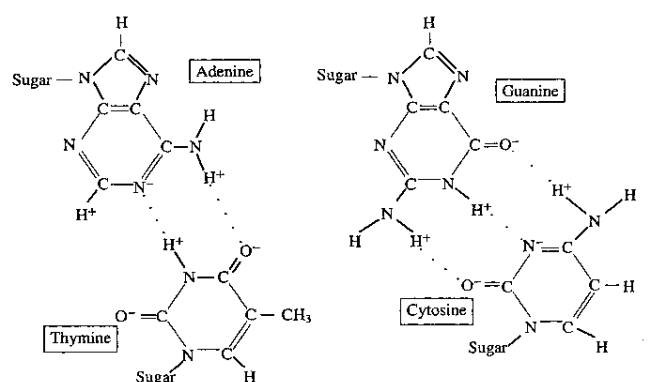
\includegraphics[width=0.7\textwidth]{images/pair-watson-crick.png}
    \caption{Extraído de \cite{nucleic-acid} para representar as ligações entre as bases nitrogenadas. }
    \label{fig:pair-watson-crick}
\end{figure}

\subsection{Mecanismo molecular e síntese protéica}

O mecanismo celular reconhece o início de um gene ou agrupamento de genes graças ao promotor, que
é uma região antes de cada gene no DNA que serve de indicação ao mecanismo celular que um gene está à frente. Tendo reconhecido o início de um gene ou agrupamento de genes, uma cópia do gene é feita em uma molécula de RNA. Este RNA resultante é o RNA mensageiro (\textit{mRNA}) e terá exatamente a mesma sequência que uma das fitas do gene, mas substituindo a base nitrogenada U por T. Esse processo é chamado de transcrição. O mRNA resultante será então usado em estruturas celulares chamadas ribossomos para fabricar uma proteína. 

Como o RNA é de fita simples e o DNA é de fita dupla, o mRNA produzido é idêntico em sequência a apenas uma das fitas gênicas, sendo complementar à outra fita - tendo em mente que T é substituído por U no RNA. A fita que se parece com o produto de mRNA é chamado de fita \textit{antisense} ou codificadora, e a outra é a fita \textit{sense} ou anticodificação ou então fita molde. A fita molde é a que realmente é transcrita, pois o mRNA é composto pela união de ribonucleotídeos complementares a esta fita.

A proteina é uma macromolécula formada por uma cadeia de aminoácidos pareadas por uma ligações peptídicas que conectam um átomo de carbono pertencente à carboxila a um ou mais átomos de nitrogênio. Ao efetuar a ligação, uma molécula de água é liberada porque o oxigênio e o hidrogênio da carboxila se une a um hidrogênio do grupo de amina. Assim, o que realmente encontramos dentro de uma cadeia polipeptídica é um resíduo do aminoácido original. As proteínas típicas contêm cerca de 300 resíduos, mas existem proteínas com apenas 100 ou com até 5.000 resíduos. \cite{nucleic-acid}
\\ \\ \\ \\ \\ \\ \\ 
\begin{figure}[h]
    \centering
    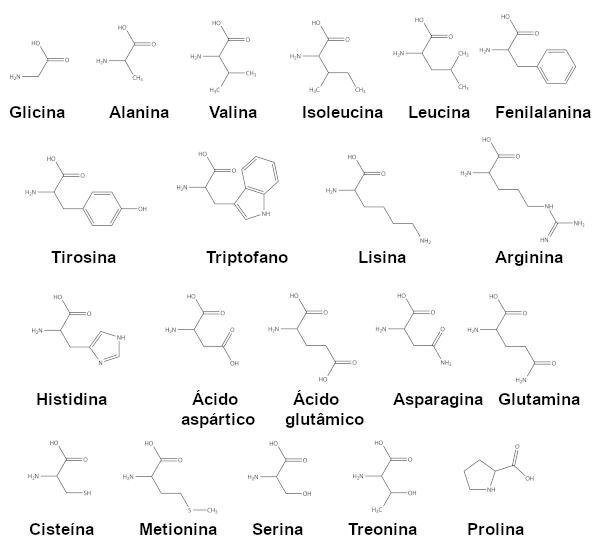
\includegraphics[width=0.65\textwidth]{images/aminoacidos.jpg}
    \caption{Moléculas de aminoácidos conhecidas.}
    \label{fig:aminoacidos}
\end{figure}

Portanto, para "especificar" uma proteína, é necessário decodificar cada aminoácido que ela contém. E isso é precisamente o que o DNA em um gene faz, usando triplas de nucleotídeos para especificar cada aminoácido. Cada tripla de nucleotídeos é chamado de códon. As triplas de nucleotídeos são dados usando bases de RNA em vez de bases de DNA, a razão é que são as moléculas de RNA que fornecem a ligação entre o DNA e a síntese protéica em um processo chamado de tradução. A conexão que designa a síntese protéica é feita entre um códon e o aminoácido que este códon codifica. Cada molécula de tRNA possui, de um lado, uma conformação que possui alta afinidade por um códon específico e, do outro lado, uma conformação que liga-se facilmente ao aminoácido correspondente. À medida que o RNA mensageiro passa o interior do ribossomo, um tRNA correspondente ao códon atual se liga a ele, trazendo o aminoácido. \cite{bio-info}

Um aspecto do processo de transcrição importante é o conceito de frame da leitura. Um quadro de leitura aberto, ou ORF, em uma sequência de DNA é um trecho contíguo dessa sequência começando no códon inicial, tendo um número inteiro de códons (seu comprimento é um múltiplo de três) tal que nenhum de seus códons seja um codão de terminação (uma tripla de nucleótidos que sinaliza a terminação da tradução). Uma das três formas possíveis de agrupar bases para formam códons em uma sequência de DNA ou RNA. Por exemplo, a sequência \textbf{TAATCGAATGGGC} pode ser decodificada tomando como códons TAA, TCG, AAT, GGG, deixando de fora o último C. Outro quadro de leitura seria ignorar o primeiro T e obter os códons AAT, CGA, ATG, GGC. Ainda outro quadro de leitura produziria os códons ATC, GAA, TGG, deixando de fora duas bases no início (TA) e duas bases no final (GC).\cite{stop-codon}

\begin{figure}[h]
    \centering
    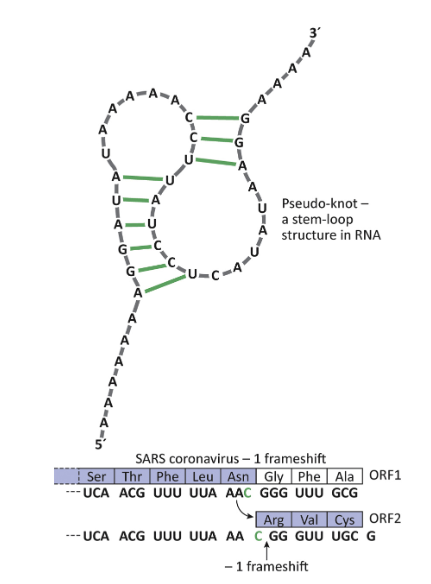
\includegraphics[width=0.65\textwidth]{images/covid_synthesis_proteic.png}
    \caption{Um pseudo-nó de RNA direcionando a estrutura ribossômica na síntese protéica. Extraído de \cite{stop-codon}}
    \label{fig:aminoacidos}
\end{figure}

\subsection{ncRNAs}

As regiões de proteínas não-codificadas abrangem 2\% do genoma humano e caracterizam por ser uma região a qual os RNAs detectados não são codificados a partir da síntese protéica. Os RNAs não traduzidos em proteínas foram nomeados RNAs não-codificadores (ncRNA) e foram considerados, a princípio, como um ruído ou subprodutos do fluxo de informação genética do DNA à proteína. A falta de dados científcos atribuindo funções para a maioria das regiões não codificantes do genoma reforça a ideia de que essa maioria pode realmente ser descartável. No entanto, hoje, é conhecido que os ncRNAs estão envolvidos em várias atividades celulares, como silenciamento de genes, replicação, regulação da expressão gênica, transcrição, estabilidade cromossômica, estabilidade de proteínas, translocação e localização, modificação de RNA, processamento e estabilidade. \cite{ncRNAs-intro}.

A predição de estruturas  conservadas é um fator preponderante para descobrir e caracterizar assinaturas para uma família de RNA específica. Ao tratar sobre ncRNAs, a sua identificação está
estritamente ligada à sua estrutura terciária e, como a estrutura terciária é determinada pela estrutura secundária, esta última é usada como uma aproximação no estudo de funções em ncRNAs. Se a função de um único RNA ou de uma família não for conhecida, pode-se inferir comparando a estrutura de RNA (ou consenso no caso de uma família) com um banco de dados de assinaturas estruturais secundárias. A comparação estrutural pode também ser usada para detectar a ocorrência de diferentes estruturas estáveis para a mesma molécula (o que pode indicar uma possível mudança na estrutura secundária impactando diretamente na sua função) para prever e comparar as mutações em uma sequência de RNA. \cite{ncRNAs-mitochondrial}

\begin{figure}[h]
    \centering
    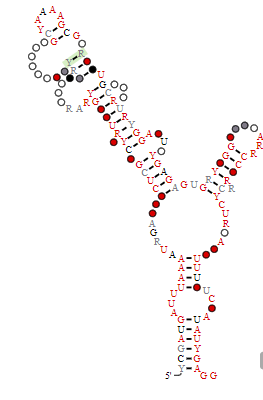
\includegraphics[width=0.5\textwidth]{images/secondary_structure_ncRNA.png}
    \caption{Estrutura secundária do icd-II ncRNA.}
    \label{fig:aminoacidos}
\end{figure}


A designação de famílias  de ncRNAs a partir da comparação estrutural secundária de sequências de ncRNAs, procurando RNAs homólogos a um candidato específico ou que pertence a uma família de candidatos continua sendo um problema específico da classificação de ncRNAs. Em tese, a pesquisa de ncRNA envolve três tipos principais de problemas de reconhecimento de padrões em ncRNas, segundo \cite{ncRNAs-content}, são eles:

\begin{itemize}
    \item Predição da estrutura secundária: O número de estruturas secundárias possíveis cresce exponencialmente com o comprimento da sequência. A questão é como buscar uma estrutura neste espaço de solução exponencial para escolher a melhor estrutura. Quando a estrutura secundária de apenas uma sequência de RNA precisa ser prevista, apenas métodos iniciais podem ser usado. Se um conjunto de RNAs homólogos estiver disponível, métodos comparativos podem prever a estrutura de consenso com mais precisão.
    
    \item Comparação de estrutura secundária: A comparação de estrutura calcula a diferença entre duas estruturas. A medição é feita calculando a diferença de uma distância de edição entre essas duas estruturas. A distância de edição depende de quantas operações de edição são necessárias para transformar uma das estruturas em outra considerando o custo de cada tipo de operação de edição. O cálculo da distância de edição está diretamente relacionada à forma como as estruturas são representadas e em que nível de resolução a comparação é realizada. Três maneiras comuns de representar estruturas são árvores, cadeias de colchetes e gráficos genéricos. Os níveis de resolução variam de pares de bases para padrões estruturais como hélices, loops e multi-loops.
    
    \item Identificação de RNA não codificadores: A detecção computacional direcionados a famílias de ncRNAs usam o máximo possível de peculiaridades. A criação de programas mais gerais que possam ser treinados para identificar características de uma família específica ou mesmo de uma única sequência de entrada é um caminho possível para identificação de famílias. Ainda assim, é desejável procurar novas famílias de genes, o que torna um problema para os programas de classificação geral de famílias conhecidas.
    
\end{itemize}

\subsection{snoRNAs}

Pequenos RNAs nucleolares (snoRNAs) são uma das mais antigas e numerosas famílias de RNAs não codificantes (ncRNAs), estão amplamente presentes nos nucléolos das células eucarióticas e têm um cumprimento de 60–300 nt. A principal função dos snoRNAs é guiar a modificação de rRNA específica do local. Em contraste, sua organização genômica e estratégias de expressão são as mais variadas. Aparentemente, as unidades de codificação de snoRNA adotaram, no curso da evolução, todas as formas possíveis de serem transcritas, proporcionando assim um paradigma único de flexibilidade de expressão gênica. \cite{snoRNAs-paradigm}

Os snoRNAs são codificados principalmente por regiões intrônicas de genes codificadores de proteínas e não codificadores de proteínas. Normalmente, podem ser classificados em três grupos: H/ACA box, C/D box e RNAs cajal pequenos (scaRNAs). Para \cite{snoRNAs-content}, os dois primeiros tipos de snoRNAs participam do processamento de RNA ribossômico (rRNA) adicionando modificações de 2-O-metilação e pseudouridilatação às moléculas de rRNA, respectivamente. No entanto, um tipo de snoRNAs estão localizados em corpos de Cajal (CBs), eles são chamados scaRNAs. Eles também seguem a classificação C/D-H/ACA, mas alguns scaRNAs contêm estruturas C/D e H/ACA. \textit{C/D box} snoRNAs se ligam a quatro proteínas essenciais – Nop1p, Nop56p,
Nop58p e Snu13p — para gerar pequenas ribonucleoproteínas nucleolar (snoRNPs). Da mesma forma, os snoRNAs de caixa H/ACA formam snoRNPs funcionais ligando-se a Cbf5p, Gar1p, Nhp2p e Nop10p.

O comprimento dos snoRNAs da \textit{C/D box} eucariótica geralmente varia de 70 a 120 nt. Esses snoRNAs contêm duas sequências conservadas: a \textit{C box e a D box}. A \textit{C box} consiste nos nucleotídeos \textbf{RUGAUGA}, que estão localizados na extremidade 5' da molécula de snoRNA. Em contraste, a \textit{D box} está localizada na extremidade 3' e consiste nos nucleotídeos \textbf{CUGA}. Juntos, esses elementos dependem do par de bases para dobrar em uma estrutura chamada \textit{kink-turn}. Essa estrutura é reconhecida pelo Snu13p, que então recruta Nop1p (também chamado fibrilarina [FBL]), Nop58p e Nop56p para modificação de 2'-O-metilação. \cite{snoRNAs-paradigm}.

\begin{figure}[h]
    \centering
    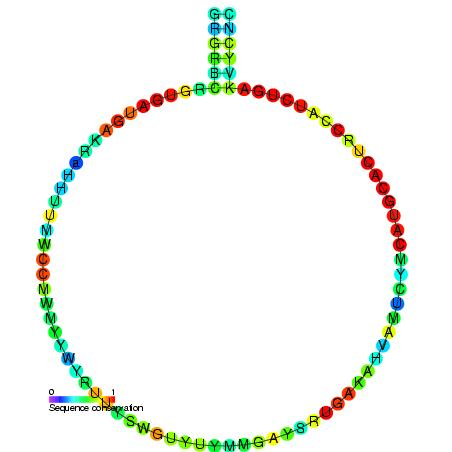
\includegraphics[width=0.5\textwidth]{images/snoRNA_c_d_box.jpg}
    \caption{Estrutura secundária do SNORD33, que pertence ao grupo \textit{C/D box}.}
    \label{fig:aminoacidos}
\end{figure}

Os snoRNAs \textit{H/ACA} geralmente têm 10 a 14 nt de comprimento e contêm a região chamada de bolsas de pseudouridilatação em que há resíduos de uridina no substrato RNA isomerizados. \textit{H/ACA box} snoRNPs se ligam a Cbf5p, Nop10p, Gar1p e Nhp2p, entre os quais
Cbf5p atua como a proteína catalítica envolvida na pseudouridilatação. Os snoRNAs eucarióticos H/ACA box contêm duas sequências: a \textit{H box} e a \textit{ACA box}, localizadas abaixo do primeiro e segundo \textit{hairpin}, respectivamente. \cite{snoRNAs-paradigm}.

\begin{figure}[h]
    \centering
    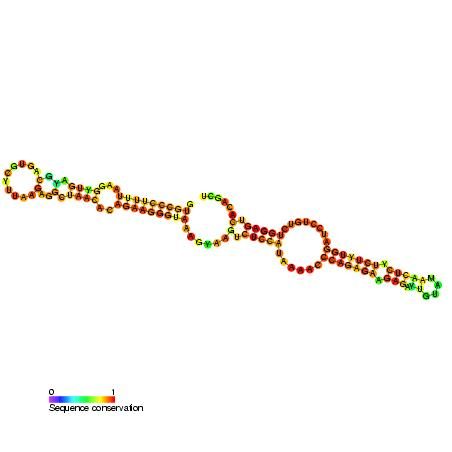
\includegraphics[width=0.5\textwidth]{images/snoRNA_h_aca_box.jpg}
    \caption{Estrutura secundária do SNORA26, que pertence ao grupo \textit{H/ACA box}.}
    \label{fig:aminoacidos}
\end{figure}


\section{\textit{Machine learning}}

De acordo com \cite{ml-approach}, o \ac{ml} é um ramo da inteligência artificial que envolve a autoaprendizagem do computador para executar tarefas. A seleção de características no aprendizado de máquina têm um papel significativo no desempenho dos modelos de previsão. É durante a seleção que a redundância e ruídos são identificados, a remoção do sobre-ajuste é aplicado, o que implica diretamente no aumento da velocidade de cálculo. Esta etapa crucial é capaz de definir as características discriminantes do objeto de estudo analisado.  Para entender melhor, o autor Mitchell, em \cite{ml-book}, explica o funcionamento do aprendizado de máquina sugerindo uma esquematização de um programa de computador o qual aprende a partir de uma experiência E através de alguma classe de tarefas T e uma medida de desempenho P. Vale ressaltar que sua performance para a tarefa T, medida em P, é aprimorada com a experiência E. Por exemplo, considerando a aplicabilidade do objeto de estudo da tese, considere que um programa deve classificar uma determinada sequência de código genético e precisa classificá-lo como um RNA, portanto:

\textbf{O problema pode ser traduzido para:}
\begin{itemize}
    \item Tarefa \textit{T}: Classificar o código genético em DNA ou RNA
    \item Medida de desempenho \textit{P}: Percentual de sequências de RNAs classificadas corretamente
    \item Experiência \textit{E}: Um banco de dados de sequências conhecidas de DNAs e de
sequências de RNAs
\end{itemize}

Dado um conjunto de dados, o algoritmo fará o treinamento a partir das características (\textit{features}) predefinidas que descrevem o RNA. A hipótese inicial é que haja uma função \textit{f} que consiga ser aplicável à um grupo \textit{X} de código genético que o caracterize como um RNA. O algoritmo não retorna uma solução exata, logo, a correlação do resultado é baseado na margem de erro da função heurística. Todavia, a intenção do aprendizado de máquina é que torne a máquina consistente ao armazenar a "experiência" ou informação advindas do banco de dados; quanto mais características estiver disponível para definir o caso de estudo, melhor. A determinação da acurácia é feita pelo valor resultante do \textit{F-score}, em termos estatísticos, é a medida de precisão de um teste, portanto, a escolha do conjunto de dados bem como a preferência do algoritmo impactam diretamente na sua eficácia. \cite{ml-intro}


\begin{figure}[h]
    \centering
    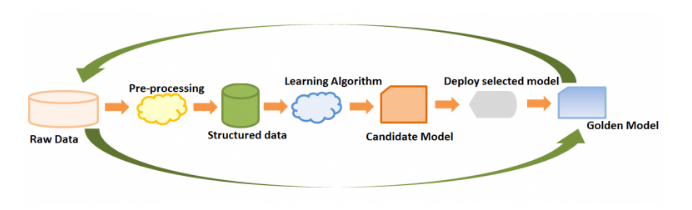
\includegraphics[width=0.8\textwidth]{images/workflow.png}
    \caption{Fluxo de trabalho do aprendizado de máquina.}
    \label{fig:workflow}
\end{figure}

A figura ~\ref{fig:workflow} mostra um simples fluxo de trabalho do aprendizado de máquina, inclusive, muito utilizado na mineração de dados: na primeira etapa recebe o dado bruto e em seguida passa para a etapa de pré-processamento que filtrará os dados e os limpará deixando-o estruturado, em sequência o algoritmo escolhido é executado e retornará o "modelo de candidado" para o treinamento em questão, a verificação do F-score é feito na fase seguinte e o "modelo de ouro", isto é, o grupo classificado que obteve a maior acurácia é encontrado. \cite{ml-intro}
O aprendizado de máquina é dividido em três grupos: aprendizado supervisionado, não supervisionado e reforçado. O aprendizado híbrido, por sua vez, combina ambos métodos: supervisionado e não supervisionado.

No estudo de \cite{ml-intro}, define-se que o aprendizado supervisionado mapeia uma entrada para uma saída com base em um conjunto de dados conhecidos, a saída é uma classe (no caso de classificação) ou um valor (em regressão linear). Na aprendizagem não supervisionada, os algoritmos construem modelos capazes de descrever os dados e as relações encontradas sem o uso de rótulos, além de incluir a divisão de dados em grupos (no caso de agrupamento) e resume a distribuição de dados em densidade estimativa. A aprendizagem por reforço envolve ações de aprendizagem em vez de classe, e a entrada é mapeada para ações com base no retorno, logo, é orientada a ação, onde são mantidas as ações que conterem maior recompensa. Para elucidar, as próximas seções abordarão alguns algoritmos de classificação importantes como \textit{SVM}, \textit{CNN} e \textit{Explicit Decomposition with Neighborhoods} (EDeN) para ilustrar alguns dos métodos disponíveis do aprendizado de máquina.

\subsection{SVM}

O SVM é um método não paramétrico que não é limitado pelo tamanho do conjunto de dados de treinamento. Essencialmente, o SVM gera modelos usados para classificação e regressão \cite{svm-1}. Em ambos os casos, se o SVM não for capaz de criar os vetores de suporte, ele pode construir hiperplanos em uma dimensão alta no espaço euclidiano para que ele selecione aqueles com maior margem, relacionados aos dados de treinamento \cite{svm-content}.  Nessas circunstâncias, o modelo SVM tenta encontrar uma reta para distinguir os grupos da entrada do conjunto de dados, excluso os casos em que as margens não podem ser criadas quando métodos simples de separação linear são usados para dados não-lineares. 

Com a finalidade de resolver este obstáculo, o SVM usa funções do kernel para aumentar a dimensão do espaço, de modo que o conjunto de dados possa ser linearmente separável em dimensões mais altas.

\begin{figure}[h]
    \centering
    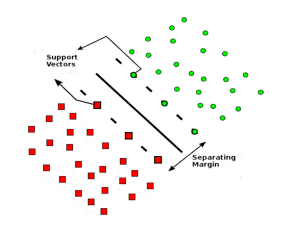
\includegraphics[width=0.5\textwidth]{images/svm_1.png}
    \caption{Exemplo de vetores de suporte de 2 dimensões adaptado por \cite{svm-content}.}
    \label{fig:svm_1}
\end{figure}

\begin{figure}[h]
    \centering
    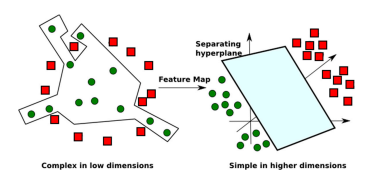
\includegraphics[width=0.5\textwidth]{images/svm_2.png}
    \caption{Dados separáveis não lineares em baixa dimensão, mapeados para uma dimensão mais alta; adaptado por \cite{svm-content}.}
    \label{fig:svm_2}
\end{figure}

Uma noção que é central para a construção do algoritmo de aprendizado do vetor de suporte é o kernel do produto interno entre um "vetor de suporte" xi e o vetor x extraído do espaço de entrada. Os vetores de suporte consistem em um pequeno subconjunto dos dados de treinamento extraídos pelo algoritmo

\subsection{\textit{CNN}}

O trabalho de Hubel e Wiesel em 1962 sobre a descoberta de atividades 
elétricas de neurônios em gatos foi pioneira para o desenvolvimento do método de aprendizagem de máquina baseada em multicamadas de neurônios, chamada de rede convolucional neural (CNN) \cite{hubel-wiesel}.Uma rede convolucional é um perceptron multicamada projetado especificamente para reconhecer formas bidimensionais com um alto grau de invariância à tradução, dimensionamento e distorção. Esta tarefa é aprendida de forma supervisionada por meio da rede cuja estrutura inclui as seguintes formas de restrições \cite{svm-content}:

\begin{enumerate}
    \item Extração de características - Cada neurônio recebe suas entradas sinápticas de um campo receptivo local na camada anterior, forçando-o a extrair características locais. Uma vez que um recurso foi extraído, sua localização exata torna-se menos importante, desde que sua posição em relação a outras características seja aproximadamente preservada.
    \item Mapeamento de extrações - Cada camada computacional da rede é composta de vários mapas de características, com cada mapa de características na forma de um plano dentro do qual os neurônios individuais são restringidos a compartilhar o mesmo conjunto de pesos sinápticos. Esta segunda forma de restrição estrutural tem efeitos benéficos como a invariância de deslocamento e redução da quantidade de parâmetros livres recebidos pelos perceptrons.
    \item Subamostragem - Cada camada convolucional é seguida por uma camada computacional que realiza média local e subamostragem, reduzindo a resolução do mapa de características. Esta operação tem o efeito de reduzir a sensibilidade da saída do mapa de características para deslocamentos e outras formas de distorção.
\end{enumerate}

\begin{figure}[h]
    \centering
    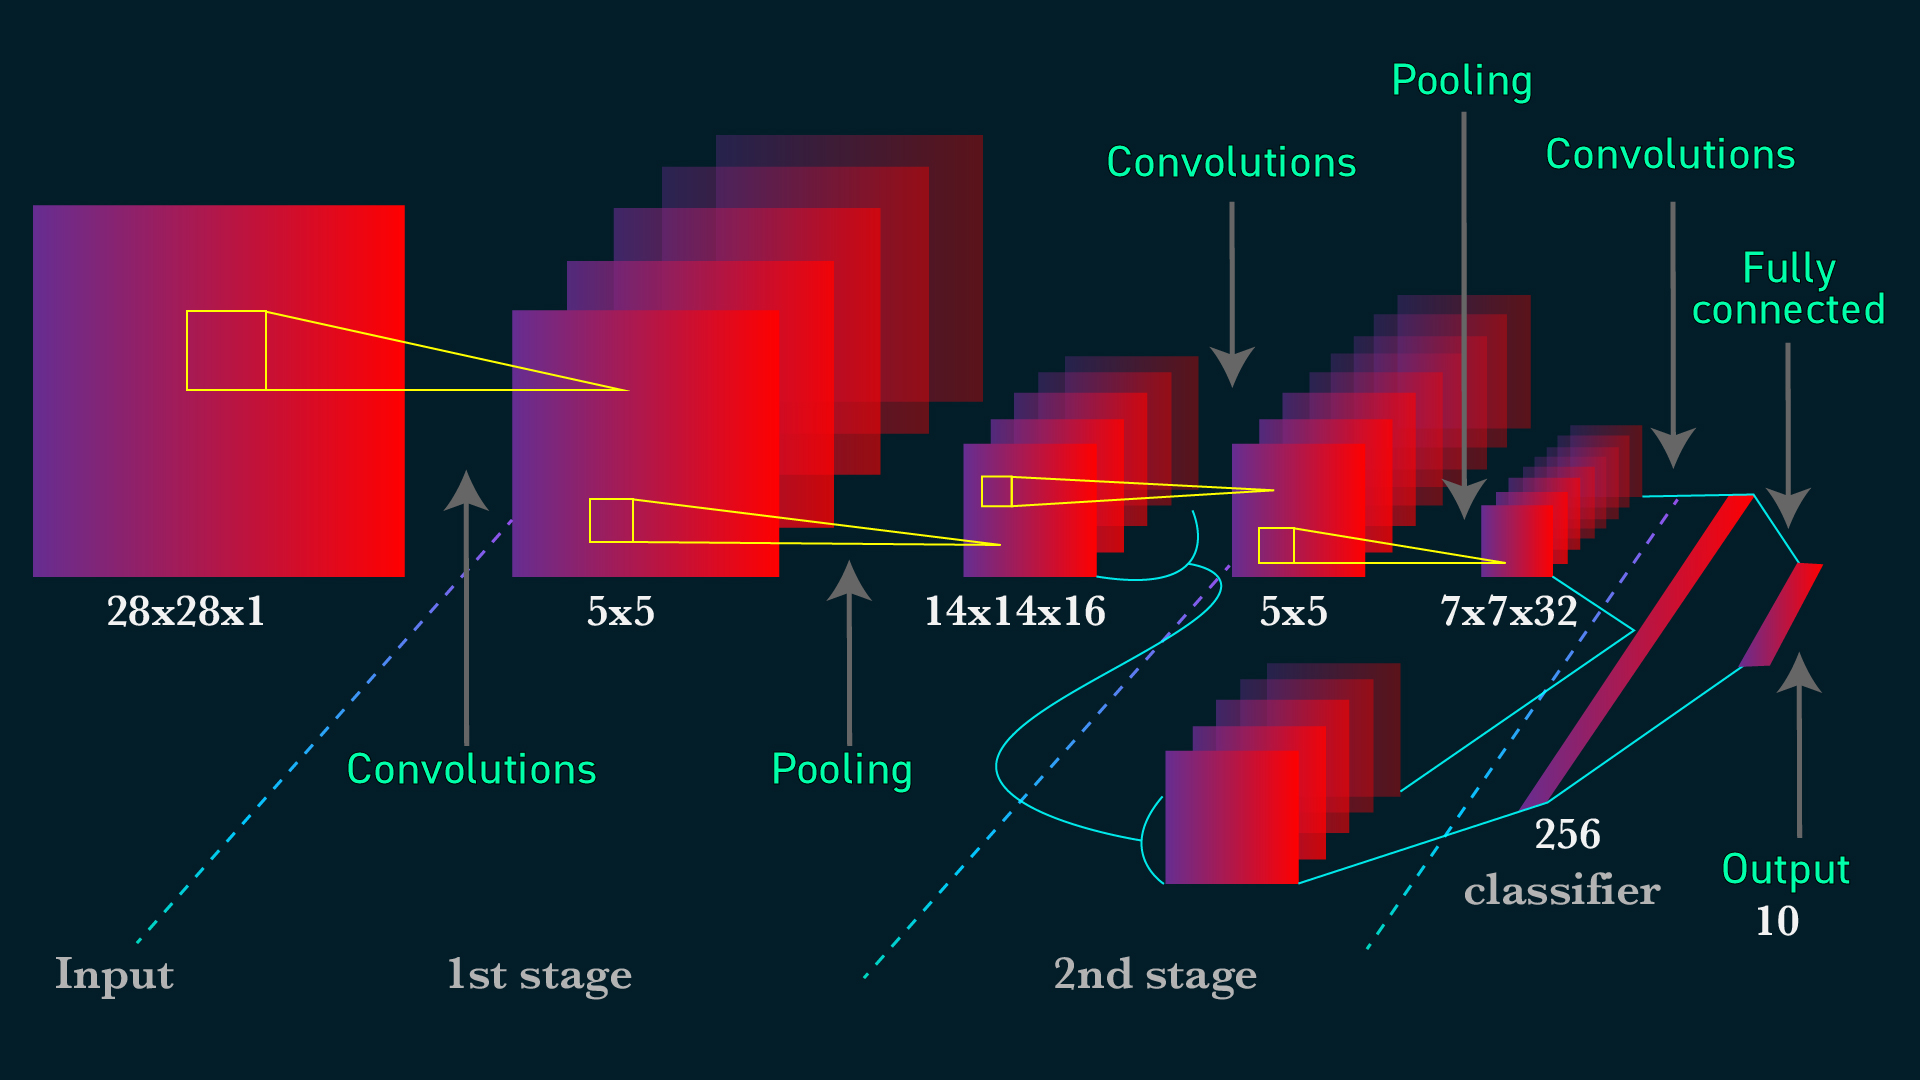
\includegraphics[width=0.55\textwidth]{images/cnn.jpg}
    \caption{Representação da rede convolucional neural no processamento de imagens (I) entrada de dados, (II) primeiro estágio, (III) segundo estágio, (IV) classificador de 256 pixels, (V) saída com 10 pixels totalmente conectada; Imagem extraída de \cite{cnn-image}.}
    \label{fig:cnn}
\end{figure}

A essência da rede neural convolucional é baseada na retropropagação que consiste na atualização contínua dos pesos para que os neurônios com a maior taxa de erro/perca sejam minimizados garantindo a consistência do modelo e a acurácia do método. A retropropagação funciona da seguinte forma: ao adentrarmos ao mapeamento de extrações, é necessário atualizar o peso de cada sináptico (ligação entre dois neurônios) de forma que aplique em todos os neurônios das camadas anteriores e para que isso seja implementado, é necessário a função de perca e a de hipótese, elas guiarão o modelo pela a rede inteira até que chegamos a uma camada final que seja utilizável \cite{cnn-blog}.

Portanto, conforme o mapeamento de extrações avança, os pesos tendem a diminuir pois são cálculos a partir da derivada parcial das funções. Consequentemente, o último nó da rede armazenará o total de perda do modelo que será usado para a avaliação do resultado, percebe-se, então, que a rede convolucional vai aprendendo a classificar o modelo por treinamento extraindo suas próprias características esporadicamente.

\subsection{EDeN}

\textit{Explicit Decomposition with Neighborhoods} (EDeN) é um kernel decomposicional de grafos baseado no \textit{Neighborhood Subgraph Pairwise Distance Kernel} (NSPDK) que produz um subgrafo da estrutura secundária do snoRNAs e produz um conjunto explícito de \textit{features} usado para algoritmos de aprendizagem de máquina supervisionados, não-supervisionados ou híbridos de maneira escalável.

A decomposição de uma sequência genômica em partes de objeto pretende conceber um kernel local válido entre as subpartes para que seja obtido uma função de similaridade capaz de decompor exponencialmente se existir um método que enumere os kernels em tempo polinomial recorrendo a programação dinâmica para tal ato. À medida que a dimensão do espaço de características torna-se maior, há uma probabilidade de que uma fração das dimensões não serão correlacionadas com a função de similaridade. Como consequência, mesmo usando algoritmos de classificação com margem alta, tornam-se obsoletos para determinar uma boa generalização do modelo. \cite{eden-nspdk}

\begin{figure}[h]
    \centering
    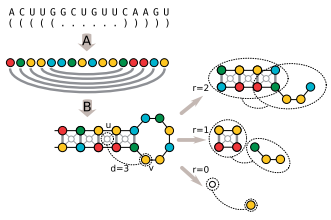
\includegraphics[width=0.6\textwidth]{images/eden_graph.png}
    \caption{\textbf{Codificação da estrutura secundária de RNA e as \textit{features} do kernel do grafo}; Imagem extraída de \cite{graph-representation}.}
    \label{fig:eden_graph}
\end{figure}

Para entender melhor como funciona a tradução da sequência para um grafo, o passo-a-passo da codificação da estrutura secundária é: \textbf{(A)} A codificação do grafo preserva a informação do nucleotídeo (rótulos do vértice) e os pares de bases (rótulos da borda), aqui representados com cores diferentes. \textbf{(B)} Vértices adicionais são inseridos para induzir \textit{features} relacionados ao empilhamento quádruplo de pares de base (vértices finos de cor cinza no centro de cada empilhamento de pares). Na parte da direita exemplo de \textit{features} induzidas pelo kernel do grafo \textit{NSPDK} para um par de vértices \textbf{u,v} na distância 3 com raio 0,1,2. Os grafos de vizinhança são encerrados em trilhas tracejadas.

Em uma conotação matemática, proposto por \cite{graph-representation}, dado um grafo $G = (V,E)$, em que $V$ é o conjunto de vértices e o $E$ é o conjunto de arestas. Sendo a distância de dois vértices $u,v$ denotada por $D(u, v)$ do menor caminho entre eles e o raio $r$ da região do subgrafo induzido é o conjunto de vértices a uma distância $d$ menor ou igual a $r$ de $v$. Considere que $N_{v,r}$ (G) denota o subgrafo de vizinhança, ou seja, o subgrafo de $G$ enraizado em $v$ induzido pelo conjunto de vértices. A relação de pares de vizinhança $R_{r,d}$ é definida como válida quando a distância entre as raízes de dois subgrafos de vizinhança de raio $r$ é exatamente igual a d. O kernel de decomposição, portanto, $k_{r,d}$ na relação $R_{r,d}$ em um NSPDK pode ser definido da seguinte forma: 

\begin{equation}
    K(G, G^{'}) = \sum_{r}^{r^{*}} \sum_{d}^{d^{*}}k_{r,d}(G, G^{'})
\end{equation}

Isto significa que o NSPDK decompõe o grafo em pares de subgrafos
vizinhos limitando a soma de $k_{r,d}$ kernels a cada iteração para todos os valores crescentes do parâmetro de raio $r$ e distância $d$ até um valor máximo dado $r^{*}$ e $d^{*}$ respectivamente.